\chapter{Bevezetés}
\pagestyle{headings}
Az 1980-as évek végén dolgozta ki Rohrer és Binning, az első mikroszkópiás módszer született a pásztázó alagút mikroszkópia (PAM, Scanning Tunneling Microscopy STM), amiért a későbbiekben Nobel-díjat kaptak, ami jelzi munkájuk jelentőségét. Az új mikroszkópiás módszer megalkotása után más pásztázó módszerek kifejlesztése is megalkotásra került. Elsőkén az atomerő  mikroszkópia (AEM, Atomic Force Microscopy AFM), majd a kémikusok által kifejlesztett pásztázó elektrokémiai mikroszkóp (PEKM, Scanning ElektroChemical Microscopy SECM). Az elekrokémiai mikroszkóp kifejlesztése Alan J. Bard és munkatársainak tulajdonítható. A detektálási módszer alapján a PEKM két változata különíthető el: voltammetriás és potenciometriás. A potenciometriás PEKM vizsgálatok kivetelezése sokkal nehezebb, mint a voltammetriásoké. Ez több okra vezethető vissza. Egyrészt a mérőcsúcsként használt mikroelektródok készítése is nehezebb, mint a  voltammetriában használatos egyszerű inert fém elektród. Másrészt a potenciometriás mikroelektródok sokkal törékenyebbek, az ezekkel való munka nagy körültekintést igényel. Egy további nagy hátránya a potenciometriás mikroelektródoknak, hogy a voltammetriás mikroelektródokkal ellentétben nem teszik lehetővé a Z-irányú pozíció meghatározást. Éppen ebből kifolyólag jóval alacsonyabb potenciometriás közlemények száma. Számos olyan probléma akad azonban, amit más módszerrel nem lehet vizsgálni, ilyenek például az in situ korróziós vizsgálatok, melyek során általában egy konkrét ionféleség térbeli aktivitás eloszlására vagyunk kíváncsiak egy korrodálódó minta felett. Egy másik jó példa a hidrogén-ion térképezése olyan folyamatokban, melyekben a pH erősen függ a térkoordinátáktól. Éppen ezért érdemes a potenciometriás PEKM fejletésével foglalkozni.
2017-ben kapcsolódtam be a Pécsi Tudományegyetem Általános Fizikai Kémia Tanszék ez irányú kutatásaiba. A potenciometriás PEKM egy új lehetséges alkalmazási területének hatékonyságát vizsgáltam. Munkámban a folyadékfázis felületének potenciometriás térképezését kíséreltem meg. A PEKM technika az esetek túlnyomó többségében elektrolitban lévő szilárd felületek vizsgálatára alkalmas. A folyadékfázis felületének PEKM térképezése egy eddig még nem vizsgált alkalmazási lehetőség, mely több érdekes folyamat vizsgálatát teszi lehetővé. Példaként a Belouszov- Zsabotyinszkij (BZ) reakciót használtam. A térkoordináta függvényében mértem a redoxpotenciált a reakció elegy felületén. A kvázi kétdimenziós keveretlen BZ reakció elegyben vertikális koncentráció változással nem kell számolni, ezért Z-irányú térképezésre nem volt szükség. Továbbá ugyanezen okból kifolyólag elegendő a legfelső 1 mikrométer vastagságú oldat réteg térképezése. További kisérleti előnyt jelent a folyadékfázis tökéletes simasága. Ezenkívül, mivel a mikroelektród csak 1 mikrométeres mélységbe hatol az oldatba, szigetelésre nem volt szükség. Ez jelentősen kisebb méretű mikroelektród készítését tette lehetővé, mely igencsak fontos a keveretlen reakció vizsgálata során, hiszen minél kisebb a mikroelektród, annál kisebb konvektív hatássa van mozgás közben. Dolgozatomban bemutatom  az első potenciometriás tér-idő képet a BZ-reakcióról és összehasonlítom a már jól ismert opikailag készült tér-idő kép.
 

A használt mérési elrendezés a \ref{fig:secm}. ábrán látható.



\begin{figure}[h]
\centering
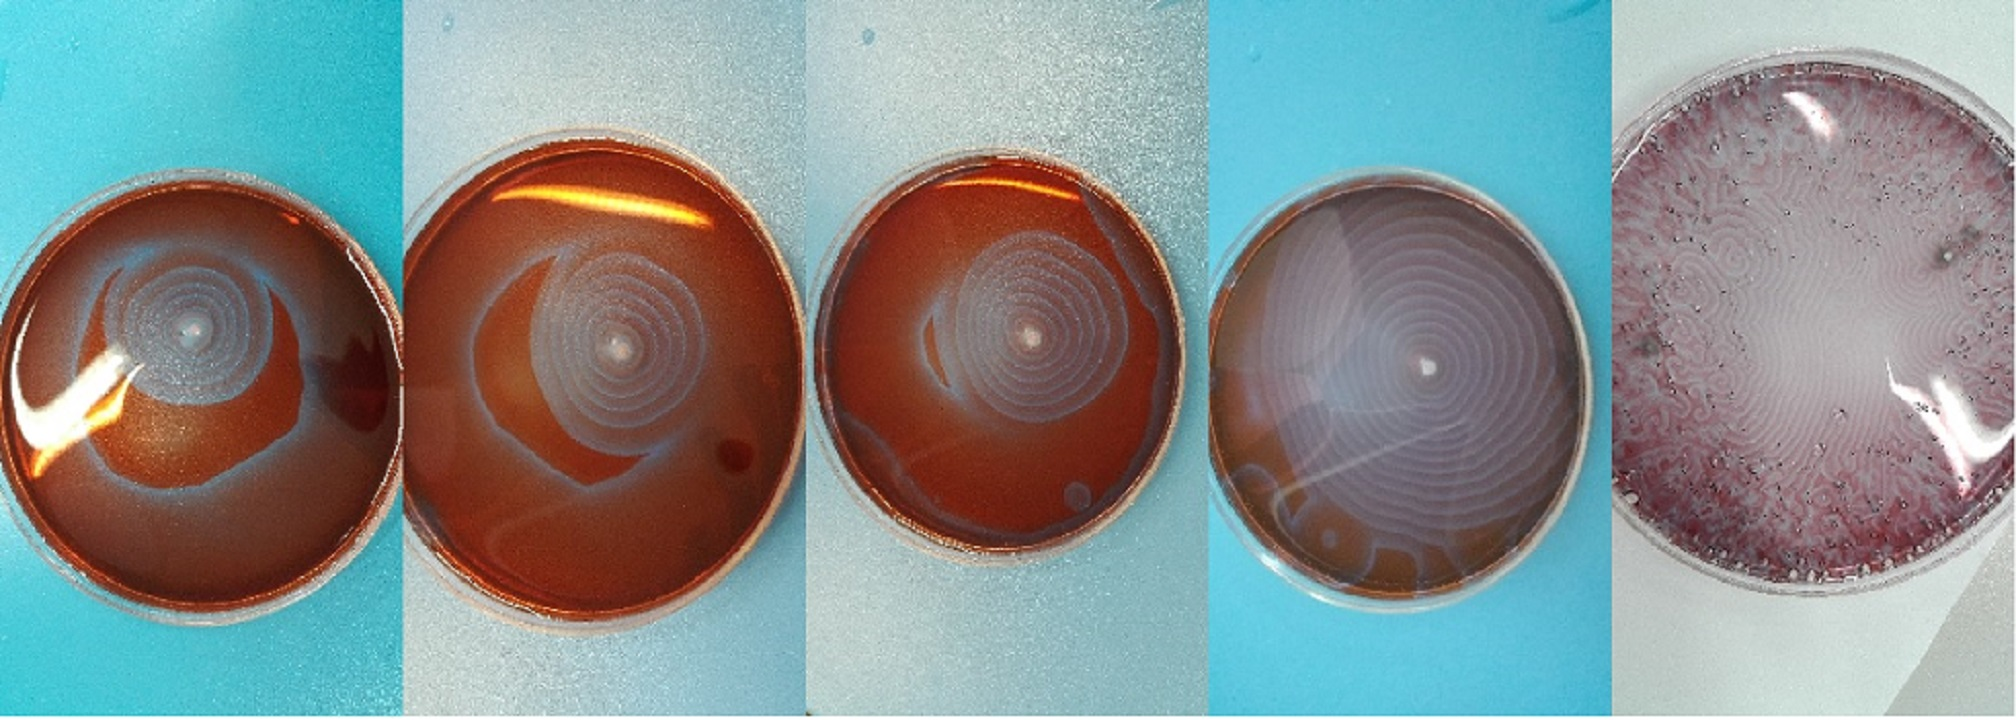
\includegraphics[width=0.8\textwidth]{img/oscillating_reaction.jpg}
\caption{(A) Valinomycin, (B) bis-N,N-dicyclohexyl-malonamide, and (C) nonactin, ionophores for potassium, magnesium, and ammonium ions, respectively.}
\label{fig:ionophores}
\end{figure}

\begin{figure}[h]
\centering
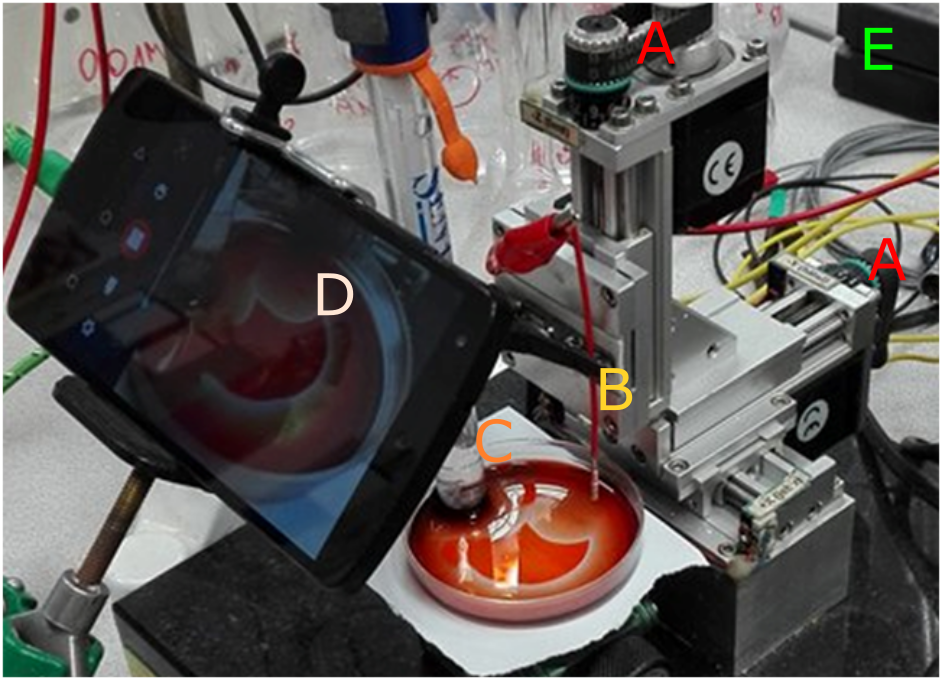
\includegraphics[width=0.8\textwidth]{img/secm.png}
\caption{(A) Léptetőmotorok, (B) indikátor elektród (C) referencia elektród, (D) kamera, (E) nagy bemeneti impedanciájú feszültségmérő.}
\label{fig:secm}
\end{figure}

\begin{table}[]
\centering
\caption{A reakció komponenseinek koncentrációi.}
\label{my-label}
\begin{tabular}{llllll}
Komponens                       & Malonsav & Kálium-bromát & Kénsav & Mangán-szulfát & Ioncserélt víz \\
\hline
Koncentráció (M)                & 1        & 0.2           & 5      & 0.125          & -              \\
Térfogat (cm$^3$) & 12       & 9             & 11     & 6              & 1              \\
\end{tabular}
\end{table}

\def\s{0.5}
\begin{figure}
%% trim = top left bottom right
\centering
\includegraphics[trim = 15mm 60mm 0mm 30mm, clip, width=\s\textwidth, angle=-90]{img/spacetime.eps}
\caption{(A) Electrochemical space-time plot overlayed on top of the corresponding optical one.
The potential of the carbon fiber microelectrode is shown as a function of spatiotemporal coordinates.
Redox indicator was ferroin.
The optical spatiotemporal image was grayscaled to allow better visibility when overlaying the electrochemical data.
The brighter stripes correspond to the oxidizing waves.
(B) The second scan cycle.
Blue line: forward scan, red line: backwards scan.
%Note the shape of the peaks on the red curve, which is measured in the direction that is opposite to the chemical wave travel.
%The elongated portion of these peaks where the potential is decreasing, is not due to 
}
\label{fig:spatiotemporal}
\end{figure}




